 \documentclass[12pt,strict]{TrilinosUserGuide}
\usepackage{array}
    \title{Trilinos Users Guide}
\SANDsubtitle{}

\author{
Michael A. Heroux \\
James M. Willenbring\\
Computational Mathematics \& Algorithms \\
 \\
Sandia National Laboratories\\
P.O. Box 5800\\
Albuquerque, NM 87185-1110 \\
 \\
maherou@sandia.gov \\
jmwille@sandia.gov \\
}

    % There is a "Printed" date on the title page of a SAND report, so
    % the generic \date should generally be empty.
    \date{\today} % Remove ``\today'' in final version


\SANDnum{SAND2003-xxxx}
\SANDprintDate{April 2003}
\SANDauthor{
Michael A. Heroux, James M. Willenbring, \\
Sandia National Laboratories}


\SANDreleaseType{Unlimited Release}


\SANDdistcategory{UC-999}    

\begin{document}
\maketitle
\setcounter{page}{3} % Accounts for blank page at beginning
\begin{abstract}

The Trilinos Project is an effort to facilitate the design, development,
integration and ongoing support of mathematical software libraries.
A new software capability is introduced into Trilinos as a {\it
package}.  A Trilinos package is an integral unit usually developed by
a small team of experts in a particular algorithms area such as
algebraic preconditioners, nonlinear solvers, etc.

The Trilinos Users Guide is a resource for new and existing
Trilinos users.  Topics covered include how to configure and 
build Trilinos, what is required to integrate an existing package into Trilinos
and examples of how those requirements can be met, as well as what
tools and services are 
available to Trilinos packages.  Also discussed are some common practices that 
are followed by many Trilinos package developers.  Finally, a snapshot
of current Trilinos packages and their interoperability status
is provided, along with a list of supported computer platforms.

\end{abstract}


\section*{Acknowledgement}
The authors would like to acknowledge the support of the ASCI and LDRD 
programs that funded development of Trilinos and recognize all Trilinos 
contributors: Teri Barth, Ross Bartlett, David Day, Bob Heaphy, 
Robert Hoekstra, Jonathan Hu, Tammy Kolda, Richard Lehoucq, Kevin
Long, Eric Phipps, 
Roger Pawlowski, Andrew Rothfuss, Andrew Salinger, Paul Sery, Ken
Stanley, Heidi Thornquist, Ray Tuminaro and Alan Williams.

\clearpage
\tableofcontents
\listoffigures
\listoftables

\clearpage
%The following file is also used in the Dev Guide
\section*{Nomenclature}
\addcontentsline{toc}{section}{Nomenclature}
\begin{itemize}

\item[Package]
A collection of software focused on one primary class of numerical
methods.  Also a fundamental, integral unit in the Trilinos framework.

\item[Trilinos]
The name of the project.  Also a Greek term which,
loosely translated means ``a string of pearls,'' 
meant to evoke an image that each Trilinos package is a pearl in its 
own right, but is even more valuable when combined with other 
packages.

\item[new\_package] A sample Trilinos package containing all of the
infrastructure to install a new package into the Trilinos framework.
Contains the basic directory structure, a collection of sample
configuration and build files and a sample ``Hello World'' package.

\item[Anasazi]
An extensible and interoperable framework for large-scale eigenvalue
algorithms.The motivation for this framework is to provide a generic
interface to a collection of algorithms for solving large-scale 
eigenvalue problems.

\item[AztecOO] 
Linear solver package based on preconditioned Krylov methods.  A 
follow-on to the Aztec solver package~\cite{Aztec2.1}.  
Supports all Aztec 
interfaces and functionality, but also provides significant new 
functionality.

\item[Belos] A Greek term meaning ``arrow.'' Belos is the next
generation of iterative solvers.  Belos solvers are written using
``generic'' programming techniques.  In other words, Belos is written
using TSF abstract interfaces and therefore has no explicit dependence
on any concrete linear algebra library.  Instead, Belos solvers can be
used with any concrete linear algebra library that implements the TSF
abstract interfaces. 

\item[Ifpack] 
Object-oriented algebraic preconditioner, compatible with 
Epetra and AztecOO.  Supports construction and use of parallel
distributed memory preconditioners such as overlapping Schwarz domain
decomposition, Jacobi scaling and local Gauss-Seidel relaxations.

\item[Komplex] 
Complex linear equation solver using equivalent real 
formulations~\cite{DayHero2000}, built on top of Epetra and AztecOO.

\item[Meros]
Segregated preconditioning package.  Provides scalable block
preconditioning for problems that couple simultaneous solution
variables such as Navier-Stokes problems.

\item[ML]
Algebraic multi-level preconditioner package.  Provides scalable
preconditioning capabilities for a variety of problem classes.

\item[NOX]
A collection of nonlinear solvers, designed to be easily integrated
into an application and used with many different linear solvers.

\item[Petra]
A Greek term meaning ``foundation.''  Trilinos has three Petra 
libraries: Epetra, Tpetra and Jpetra that provide basic classes 
for constructing and manipulating matrix, graph and vector
objects.  Epetra is the current production version that is
split into two packages, one core and one extensions.

\item[TSF]
Composed of several packages.  Thyra provides 
a basic collection of abstract interfaces to vectors, linear
operators, solvers, etc.  These interfaces provide a common
interface for applications to access one or more packages that
implement the abstract interface.  These interfaces can also be used
by other packages in Trilinos to accomplish the same purpose.
TSF Extended builds on top of Thyra, providing implicit
aggregation capabilities and overloaded operators.

\end{itemize}



\section{Introduction}
\label{Section:Introduction}
The Trilinos Project is an effort to facilitate the design, development,
integration and ongoing support of mathematical software libraries.  Trilinos 
also provides a set of core utility libraries
that provide common vector, graph and matrix capabilities, as well as
a common abstract interface for applications to access any appropriate
Trilinos package.

The overall objective of Trilinos is to promote rapid development and
deployment of high-quality, state-of-the-art mathematical software in
an environment that supports interoperability of packages while
preserving package independence. 

The Trilinos Users Guide is meant to assist new and existing
Trilinos users.  Topics covered include how to configure, build, and install
Trilinos, as well as how to run tests to insure proper installation.  In 
addition, issue reporting and how to sign up for and use Trilinos mail lists 
are discussed.  Finally, directions for obtaining Trilinos itself and 
documentation for individual Trilinos packages are provided.

%LIST OF POSSIBLE TOPICS: How to run tests,
%how to submit bug rpt, how to use mail lists - also list mail lists that 
%users are interested in.  Brief description of packages, point to package
%documentation.  How to obtain Trilinos.

For a higher-level view of the Trilinos project, please see An Overview
of the Trilinos Project~\cite{Trilinos-Overview}.  A document is also 
available specifically for Trilinos developers; please see the Trilinos 
Developers Guide~\cite{Trilinos-Dev-Guide}.  The Developers Guide contains 
both tutorial and general reference material.  

The current set of packages in Trilinos is shown in 
Figure~\ref{Figure:TrilinosPackages}.

\begin{figure}
\begin{center}
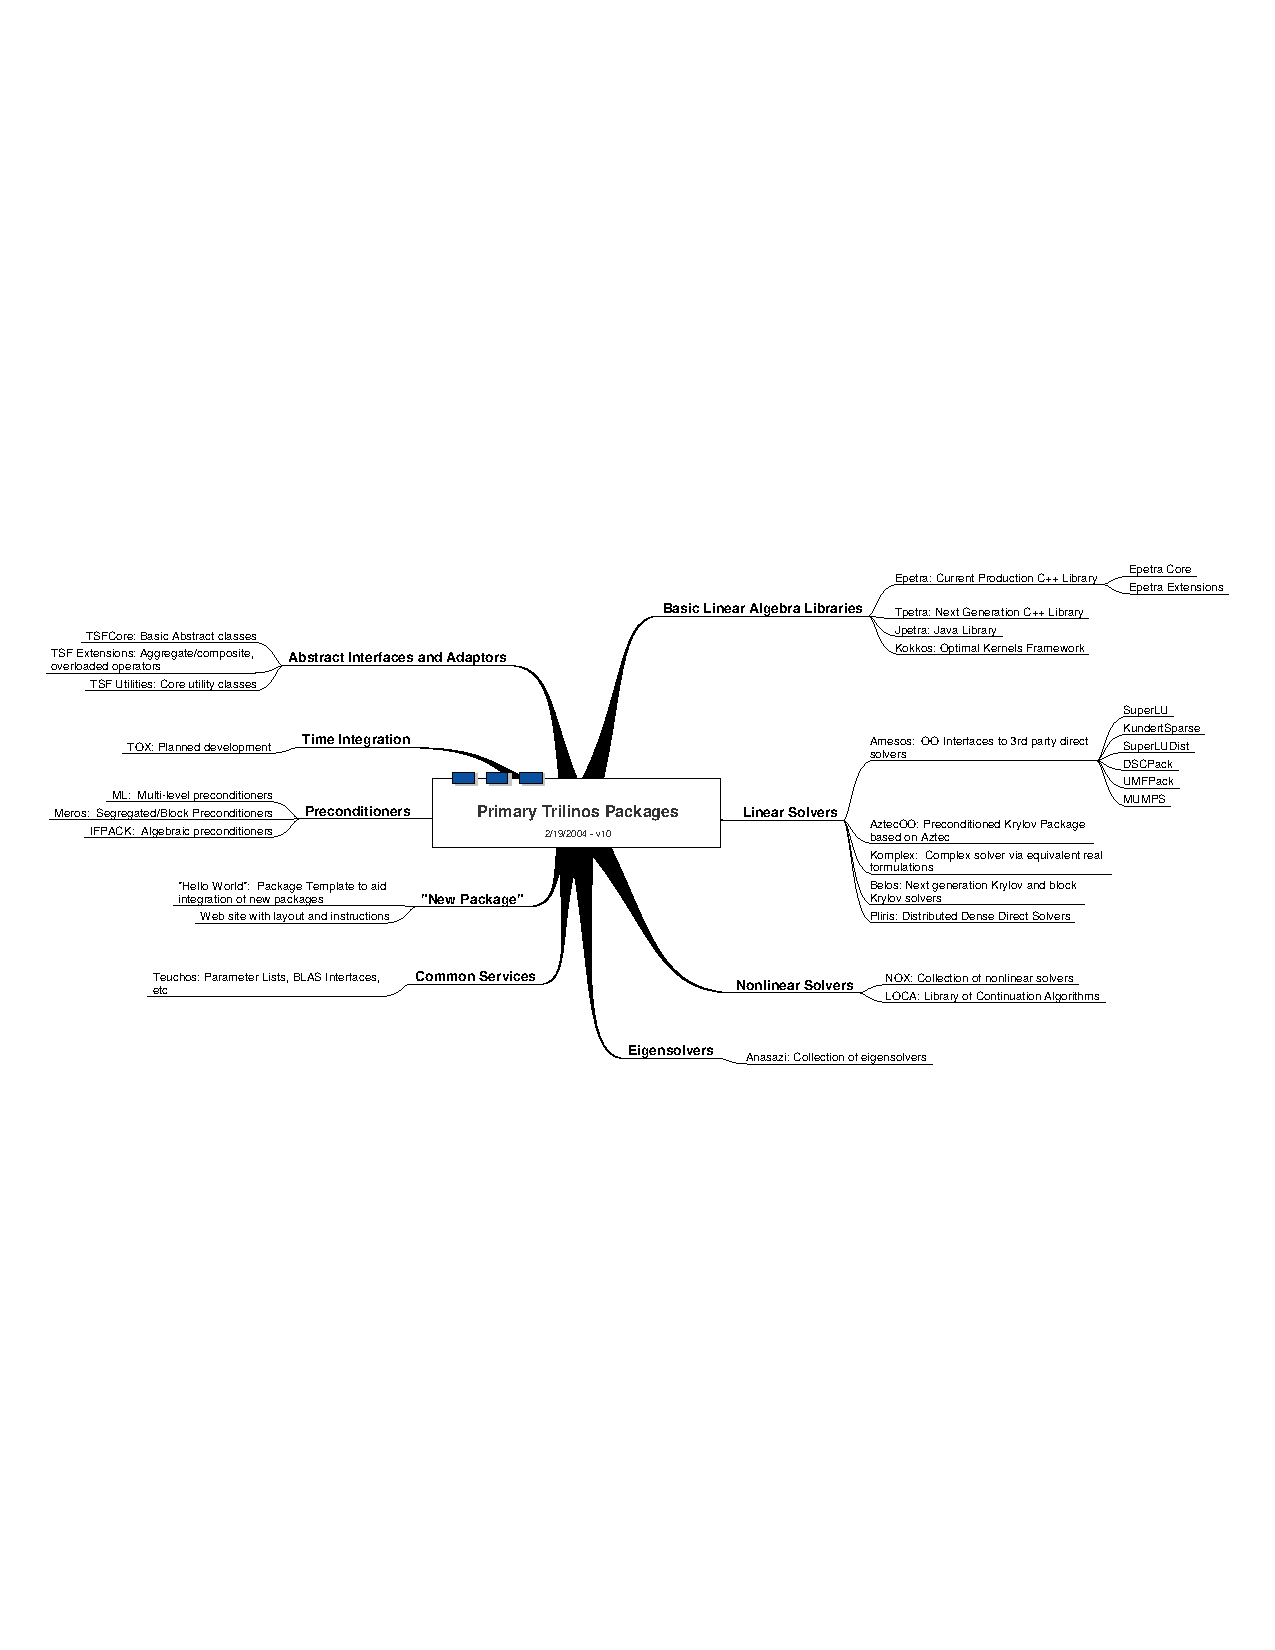
\includegraphics[height=9in]{../CommonFiles/TrilinosPackagesDiagram}
\end{center}
\label{Figure:TrilinosPackages}
\caption{Current collection of Trilinos Packages}
\end{figure}

\subsection{Typographical Conventions}

Our typographical conventions are found in
Table~\ref{Table:TypoConventions}.
\begin{table}[ht]
\scriptsize
\begin{center}
\begin{tabular}{|l|l|p{2.0in}|} \hline
Notation & Example & Description \\ \hline
\InlineCommand{Verbatim text} & \InlineCommand{../configure --enable-mpi} & 
Commands, directory and file name examples, and other text associated
with text displayed in a computer terminal window. \\ \hline
\InlineCommand{CAPITALIZED\_TEXT} & \InlineCommand{CXXFLAGS} & 
Environment variables used to configure how tools such as compilers behave. \\ \hline
\InlineCommand{[text in angle brackets]} & \InlineCommand{../configure
<user parameters>} & 
Optional parameters. \\ \hline
\end{tabular}
\end{center}
\caption{\label{Table:TypoConventions} Typographical Conventions for This Document.}

\end{table}


\section{Getting Started}
\label{Section:GettingStarted}
This chapter covers some of the basics that a user will need to know when 
beginning to work on the Trilinos project.  We address how to configure and 
build Trilinos, as well as how to add files to an existing package.

%Four subsections common to the Dev Guide and User Guide: Recommended 
%Build Directory Structure, Configuring Trilinos, Building Trilinos,
%and Trilinos Configuration Options
\subsection{Recommended Build Directory Structure}

Via Autoconf and Automake the Trilinos configuration facilities
provide a great deal of flexibility for configuring and building the
existing Trilinos packages.  However, unless a user has prior experience
with Autotools, we recommend the following process to build and
maintain local builds of Trilinos.

To start, we defined two useful terms:
\begin{itemize}
\item Source tree - The directory structure where source files are found.  A source 
tree is obtained by expanding a distribution tar ball, or by checking 
out a copy of the Trilinos repository.  
\item Build tree - The directory structure where object and library files, as well 
as executables are located.  
\end{itemize}
 
\begin{minipage}[c]{\textwidth}

\begin{minipage}[l]{.6\textwidth}

Although it is possible to run \InlineCommand{./configure} from the source tree (in 
the directory where the configure file is located), we recommend 
separate build trees.  The greatest advantage to having a separate 
build tree is that multiple builds of the libraries can be maintained
from the same source tree.  For example, both serial and parallel libraries
can be built.  
This approach also eliminates problems with configuring in a 'dirty'
directory (one that has already been configured in).
\end{minipage}\hfill
\framebox{\begin{minipage}[r]{.35\textwidth}{
{\bf Key Point:}
$\ldots$ we recommend 
separate build trees $\ldots$ multiple builds of the
libraries can be maintained from the same source tree $\ldots$ 
problems with configuring in a 'dirty' directory (are eliminated) $\ldots$
}\end{minipage}}
\end{minipage}

Setting up a build tree is straight-forward.
Figure~\ref{Figure:TrilinosDirectoryStructure} illustrates the
\begin{figure}
\begin{center}
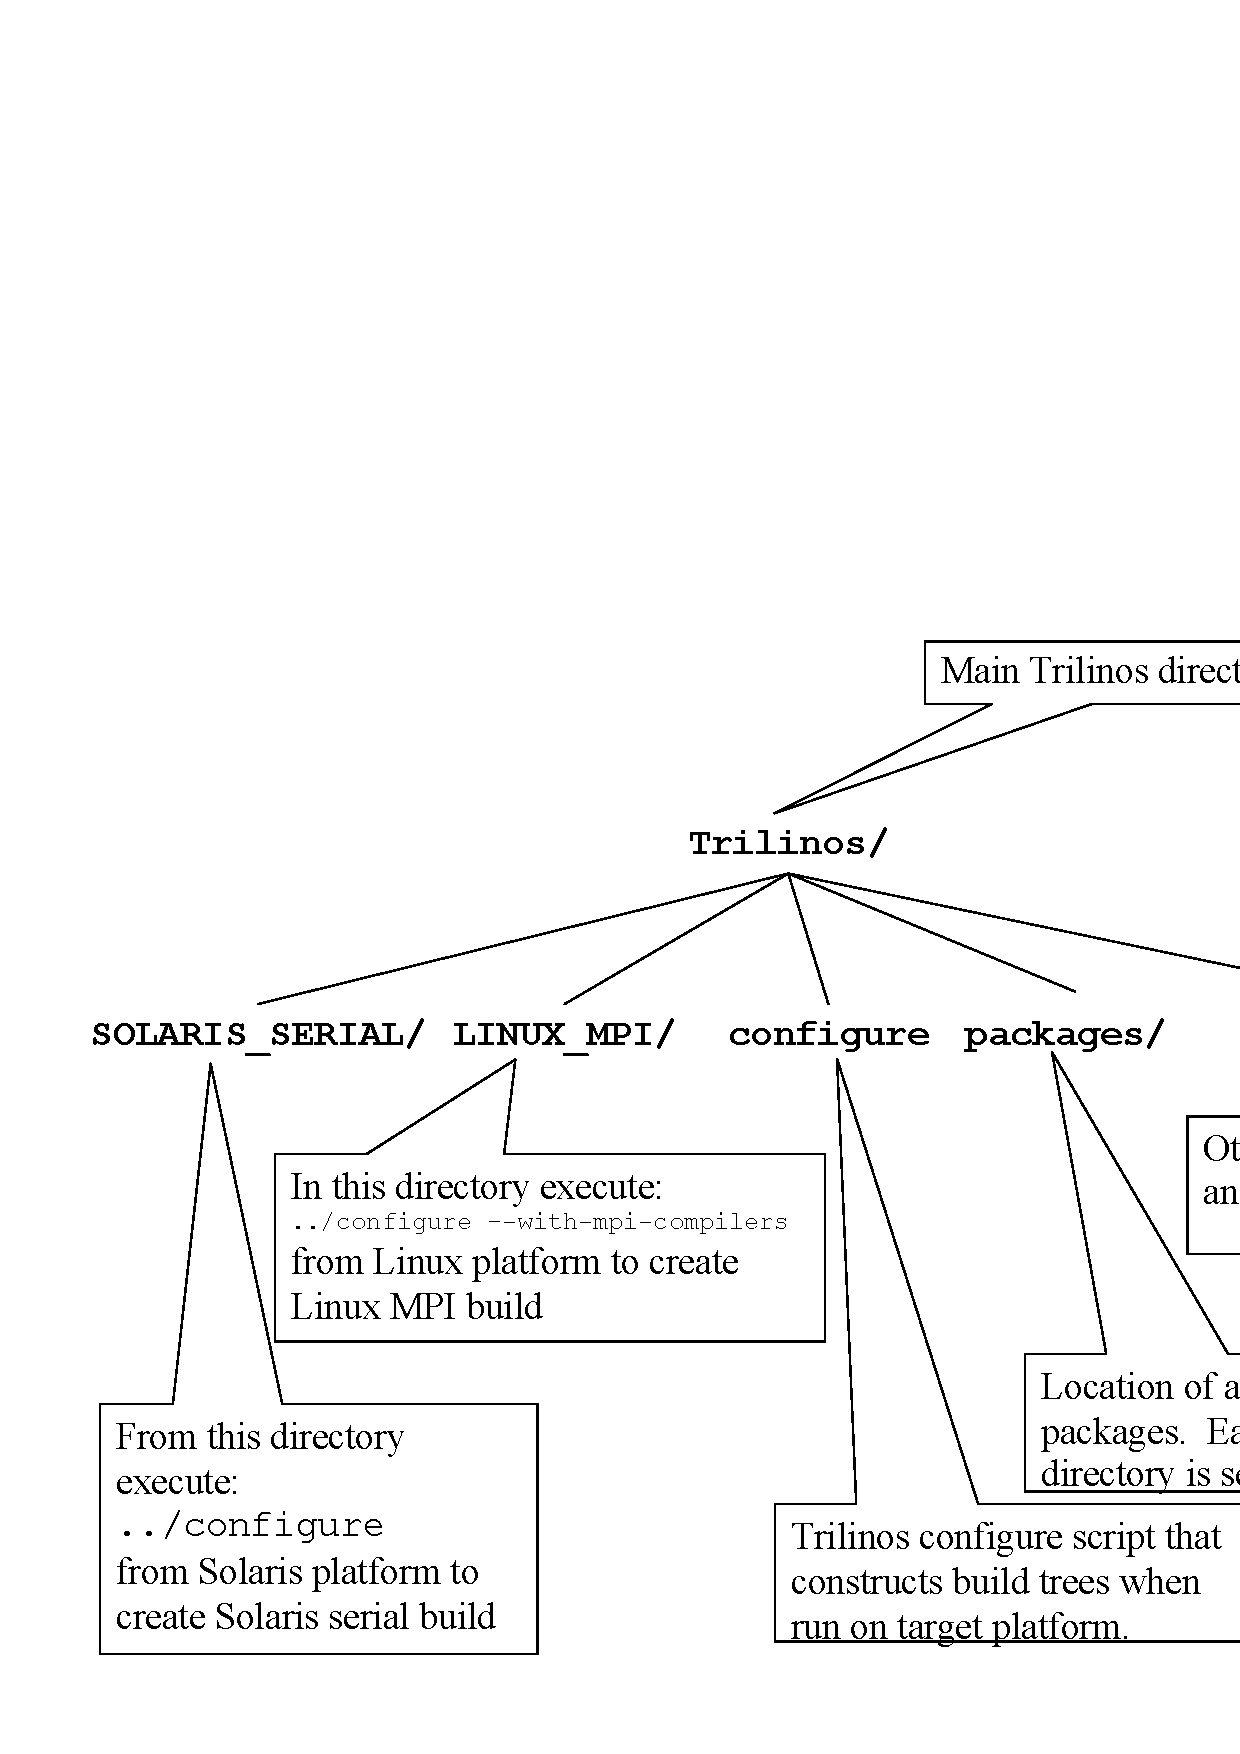
\includegraphics[width=6in]{../CommonFiles/TrilinosDirectoryStructure}
\end{center}
\caption{\label{Figure:TrilinosDirectoryStructure}Recommended Layout for Trilinos Build Directories}
\end{figure}recommended layout.  First, from the highest 
directory in the source tree (Trilinos for a repository copy, Trilinos-3.0.2 
for a distribution), make a new directory - for an MPI build
on a Linux platform, a 
typical name is \InlineDirectory{LINUX\_MPI}.  
Finally, from the new directory, type

\DisplayCommand{../configure --with-mpi-compilers}

(Note that various configure options might be necessary, see Section~\ref{Subsection:ConfiguringTrilinos} for details.)  Finally, type

\DisplayCommand{make}


In summary:

\begin{verbatim}
       cd Trilinos
       mkdir LINUX_MPI
       cd LINUX_MPI
       ../configure --with-mpi-compilers
       make
\end{verbatim}
At this point, the MPI version of Trilinos on a Linux platform is
built and completely contained in the \InlineDirectory{LINUX\_MPI}
directory.  No files outside this directory have been modified.  This
procedure can be repeated for any number of build targets.

{\bf Note:} Although we recommend the above location for build trees,
they can be set up anywhere.

\subsection{Configuring Trilinos}
\label{Subsection:ConfiguringTrilinos}

\begin{minipage}[c]{\textwidth}

\begin{minipage}[l]{.6\textwidth}

The most common issue encountered when configuring Trilinos is that it is 
nearly impossible to determine what caused configure to fail based on the 
standard output.  If the output from configure is inadequate, 
look at the config.log file (in the buildtree)
for the package that failed to configure properly.  

\end{minipage}\hfill
\framebox{\begin{minipage}[r]{.35\textwidth}{
{\bf Key Point:}
$\ldots$ to determine what caused configure to fail $\ldots$ 
look at the config.log file $\ldots$
}\end{minipage}}
\end{minipage}

To determine which 
package failed to configure, look at the bottom of the output from the 
\InlineCommand{configure} command.  One of the last lines will say something 
like:

\begin{verbatim}
    configure: error: /bin/sh '../../../packages/epetra/configure'
    failed for packages/epetra
\end{verbatim}

This particular error indicates to look in 
\InlineDirectory{packages/epetra/config.log}.

	To configure from a remote build tree, simply run the configure script 
in source tree from the root of the build tree.  In the example above, cd to 
the SOLARIS\_SERIAL directory and type 
\DisplayCommand{../configure <configure options>}

A detailed list of configure options can be seen by typing
\DisplayCommand{./configure --help=recursive} from the top level of the 
source tree.  This will display the help page for the Trilinos level as well as all 
Trilinos packages that use Autoconf and Automake.  The output from this command
is quite extensive.  To view the help page for an individual package, cd to 
the home directory for the package in the source tree and type 
\DisplayCommand{./configure --help} 
This command will also display the help page for Trilinos level 
options when used from the Trilinos home directory in the source tree.


Many of the Trilinos configure options are used to describe the details of the 
build.  For 
instance, serial or mpi, all of the packages, or just a proper subset.  

To configure for serial libraries, no action is necessary,
but to configure for parallel libraries, a user must append appropriate 
arguments to the configure invocation line as described in ``Trilinos 
Configuration Options'', section~\ref{subsect:TrilinosConfigOptions}.

Also, to build the default set of Trilinos libraries, no action is 
necessary, but to exclude a package that is built by default, Komplex for 
example, append \newline \InlineCommand{--disable-komplex} to the configure 
invocation  line.  Similarly, to include a package that is not currently built 
by default, NOX for example, append \InlineCommand{--enable-nox} to 
the configure invocation line.  It is recommended that users always configure 
from the Trilinos level and use \InlineCommand{--disable-<package>} as 
necessary, rather than trying to configure from a lower level.  To see which 
packages are built by default and which ones aren't, simply cd to the Trilinos home directory and type \DisplayCommand{./configure --help}


{\bf NOTES:} 
\begin{enumerate}
\item {\bf Enabling/Disabling package builds:} 
The configure process is set up to detect when a 
\InlineCommand{--disable-<package>} option would break a package dependency.  
For example, Ifpack depends on Epetra, so if a user wants to build Ifpack, but 
types \InlineCommand{--disable-epetra}, Epetra will be configured and built 
anyway.  

\item {\bf Installing libraries and header files:}
To install libraries and header files in a particular location, 
use \InlineCommand{--prefix=<dir>} on the configure line.  If this option is 
used, libraries will be located in \InlineDirectory{<dir>/lib} and header files in 
\InlineDirectory{<dir>/include/<package>}.

\item {\bf Providing additional information to Autotools:}
Although Autotools will try to determine all configuration
information, the user must provide anything that Autotools needs and 
cannot find.  Also, if Autotools selects, for example, the wrong 
BLAS library by default, the user must indicate which BLAS library to use.  
Other issues such as standards 
non-compliance are also dealt with here.  If all required libraries (often 
the BLAS and LAPACK) are located in standard places and no special 
compiler flags are required, try configuring without
providing additional information.

\item {\bf Sample configure invocation scripts:}

\begin{minipage}[c]{\textwidth}
\begin{minipage}[l]{.6\textwidth}

Sample configure invocation scripts for a wide variety of platforms can be 
found in \InlineDirectory{Trilinos/config}.  These scripts are 
named using the following convention: \InlineCommand{arch\_comm\_machine}.
For example, \InlineCommand{sgi64\_mpi\_atlantis}.  
\end{minipage}\hfill
\framebox{\begin{minipage}[r]{.35\textwidth}{
{\bf Key Point:}
Sample configure invocation scripts for a wide variety of platforms can be 
found in \InlineDirectory{Trilinos/config}.
}\end{minipage}}
\end{minipage}

Note that these scripts 
are examples only and are primarily useful for the values of options such as 
\InlineCommand{LDFLAGS}, \InlineCommand{CPPFLAGS}, 
and \InlineCommand{CXXFLAGS}.  Do not expect to be able to find a 
script that can be used without modification; try to find a script for a 
similar machine to use as a guide.  

The scripts in the 
repository are not always up to date.  If a user submits a script for a 
machine that few Trilinos developers have an account on, that script may 
become obsolete if it is not updated by the user who submitted it.

Users who create scripts for other machines are encouraged to check them into 
the repository for the benefit of other users.  Users who do not have access to
the repository can send scripts to the Trilinos Library Manager.

The following is an example configure invocation script for an SGI machine:

\begin{verbatim}
../configure --enable-mpi --with-mpi-libs=-lmpi \
--with-cflags=-64 --with-fflags=-64 \
--with-cxxflags="-64 -LANG:std  -LANG:ansi-for-init-scope=ON \
-ptused -DMPI_NO_CPPBIND" \
LDFLAGS=" -64 -L/usr/lib64/mips4/r10000 -L/usr/lib64/mips4 \
-L/usr/lib64 " \
--enable-epetraext --enable-new_package \
--disable-komplex --enable-tsfcoreutils
\end{verbatim}
\end{enumerate}

\subsection{Trilinos Configuration Options}
\label{subsect:TrilinosConfigOptions}
The following options apply to all Trilinos packages unless 
an option doesn't make sense for a particular package (for example, a 
package that does not include any Fortran code will not be sensitive to 
\InlineCommand{F77=g77}), or otherwise noted.  For options specific to 
an individual package, cd to the home directory of the 
package and type \DisplayCommand{./configure --help}.

Basic Options

\begin{itemize}
\item \InlineCommand{--enable-debug} 

(NOX only.)  This turns on compiler debugger flags. It has 
not been fully tested. As an alternate, specify CXXFLAGS on the 
                 configure line.

\item \InlineCommand{--enable-opt}

(NOX only.)  This turns on compiler optimization flags. It 
has not been fully tested. As an alternate, specify CXXFLAGS on the 
                 configure line. 

\item \InlineCommand{--with-cppflags}

Specify additional preprocessor flags (e.g., "-Dflag -Idir") 

\item \InlineCommand{--with-cxxflags}

Specify additional C++ flags 

\item \InlineCommand{--with-ldflags}

Specify additional linker flags (e.g., "-Ldir") 

\item \InlineCommand{--with-ar}

Specify a special archiver command, the default is "ar cru". 
\end{itemize}

 Influential Environmental Variables

\begin{itemize}
\item \InlineCommand{CC}

C compiler command.

\item \InlineCommand{CFLAGS}

C compiler flags.

\item \InlineCommand{CXX}

C++ compiler command.

\item \InlineCommand{CXXFLAGS}

C++ compiler flags.

\item \InlineCommand{LDFLAGS}

Specify linker flags.

\item \InlineCommand{CPPFLAGS}

C/C++ preprocessor flags.

\item \InlineCommand{CXXCPP}

C++ preprocessor.

\item \InlineCommand{F77}

Fortran 77 compiler command.

\item \InlineCommand{FFLAGS}

Fortran 77 compiler flags.
\end{itemize}

MPI-Related Options

\begin{itemize}
\item \InlineCommand{--enable-mpi}

Enables MPI mode. Defines HAVE\_MPI in the (Package)\_Config.h file. Will test 
for the ability to preprocess the MPI header file and may test ability to link 
with MPI.  This option is rarely necessary as many of the below options also 
turn MPI on.  

\item \InlineCommand{--with-mpi-compilers}

Sets CXX = mpicxx (or mpiCC if mpicxx not available), CC = mpicc and 
F77 = mpif77.  Automatically enables MPI mode.  To use compilers other than 
these, specify MPI locations with the below options.  If none of these options 
are necessary, use \InlineCommand{--enable-mpi} to enable MPI mode.  In this 
case, CXX, CC, and F77 have to be set if the correct compilers are 
not chosen by default.

\item \InlineCommand{--with-mpi=MPIROOT}

Specify the MPI root directory. Automatically enables MPI mode.  If this 
option is set, \InlineCommand{--with-mpi-incdir} and 
\InlineCommand{--with-mpi-libdir} should not be used.  
\InlineCommand{--with-mpi} is a shortcut for setting \newline
\InlineCommand{--with-mpi-libdir=MPIROOT/lib} 
and \newline \InlineCommand{--with-mpi-incdir=MPIROOT/include}.

\item \InlineCommand{--with-mpi-libdir=DIR}

Specify the MPI libraries location. Defaults to MPIROOT/lib if 
\InlineCommand{--with-mpi} is specified. If multiple directories must be 
specified, try \newline
\InlineCommand{--with-ldflags="-L<dir1> -L<dir2>"} instead. 

\item \InlineCommand{--with-mpi-libs="LIBS"} 

Specify the MPI libraries. Defaults to \InlineCommand{"-lmpi"}
 if either\InlineCommand{ --with-mpi} or 
\InlineCommand{--with-mpi-libdir} is specified.

\item \InlineCommand{--with-mpi-incdir=DIR}

Specify the MPI include files location. Defaults to \InlineDirectory{MPIROOT/include} if 
\InlineCommand{--with-mpi} is specified. If multiple directories  must be specified, try 
\newline
\InlineCommand{--with-cppflags="-I<dir1> -I<dir2>"} instead.
\end{itemize}

Developer-Related Options
\begin{itemize}
\item \InlineCommand{--enable-maintainer-mode}

Enable make rules and dependencies not useful (and sometimes confusing) to 
the casual installer.
\end{itemize}

\subsection{Building Trilinos}

If the configure stage completed successfully, just type \DisplayCommand{make}
 and then, if 
\InlineCommand{--prefix} was specified, \DisplayCommand{make install}

Other important notes about the configure and build processes.
\begin{itemize}
\item Any code that links to Trilinos should define 
\InlineCommand{HAVE\_CONFIG\_H}.

\item The ``classic'' build system and Autotools do not mix.  Trying to build 
with Autotools in a directory that contains a classic build will not work.  
Before attempting an Autotools build, the classic build object, library, and 
executable files within the source tree should be removed.

\item The build process will fail on OSX if ``DropZip'' is used to 
unzip the Trilinos tarball.  This utility truncates long file names.

\end{itemize}



\section{Tools Available for Trilinos Users}
\label{Section:AvailableTools}
A number of services exist for Trilinos packages.  Many of these services 
relate directly to the requirements and suggested practices for Trilinos 
packages.  For example, the CVS repository is discussed below, and 
Trilinos packages must make use of this repository.  Also, Bonsai, Bugzilla 
and Mailman are all tools that relate to suggested practices.  (It should be 
noted that these services are not simply meant to satisfy SQE requirements.  
Rather, Bonsai, Bugzilla and Mailman have proved to be very useful tools.  
Using these tools together, along with the CVS repository, has led to a more 
time and cost effective code development process.)  For more information about 
any of the below services, please contact the Trilinos Project Leader.

\subsection{Test Harness}
\label{subsect:TestHarness}

Trilinos packages that configure and build using Autotools can easily 
utilize the the Trilinos test harness.  The Trilinos test harness is composed 
of two components.  

One part of the test harness is used to run nightly tests on a number of 
platforms.  This portion of the test harness performs a 
\InlineCommand{cvs update} (gets the most recent source code) every night and 
then builds the libraries and runs any tests that have been integrated into 
the test harness.  

Tests that are added as ``daily'' tests are run six time a week, while 
``weekly'' tests are run once a week.  Currently the nightly test harness only 
runs on Linux, IRIX64, and DEC/OSF1, but it will eventually run on 5-8 
platforms.  Packages that have not ported to a particular platform can be 
excluded from the testing process on that platform.  Packages that do not have 
any tests integrated into the test harness can still benefit by testing that 
libraries build without errors.  

The second component of the test harness is a script that should be executed 
by users before checking updates into the repository.  This script is located 
in \InlineDirectory{Trilinos/testharness/checkin-test-harness}.  The script 
provides an easy way for users to run all of the ``daily'' tests that have 
been added to the test harness for all packages from one location.  
Instructions for running the script can be found within the script itself.

Integrating existing tests into the testharness is not difficult.  
The process is discussed in 
\InlineDirectory{Trilinos/testharness/HowToAddToTestHarness}.  
Please note that this document is a work in progress.

\subsection{CVS Repository}

Trilinos source code is maintained in a CVS~\cite{CVS} repository.  It is 
very easy to add new packages to the repository.  Packages that already use 
CVS can even retain their CVS history!  To access the repository, one must 
have an account on software.sandia.gov.  Once an account has been granted, 
set the following two environment variables (replace ``your\_user\_name'' 
with your user name on software):

\DisplayCommand{CVSROOT :ext:your\_user\_name@software.sandia.gov:/space/CVS}
\DisplayCommand{CVS\_RSH ssh}

For those not familiar with CVS, a brief discussion covering some of the most 
common CVS commands is available in~\ref{Section:CVS}.  For a more complete 
listing of CVS commands, see the Gnu CVS Home Page~\cite{CVS}.

\subsection{Bugzilla}
\label{subsect:Bugzilla}
Feature and issue reports are tracked using Bugzilla~\cite{Bugzilla}.  
Bugzilla can be found on the web at 
\InlineDirectory{http://software.sandia.gov/bugzilla}.  
A Bugzilla account is necessary for submitting bugs.  Those interested can 
sign up at the website.  All bugs related to any package of Trilnos that uses 
Bugzilla should be submitted to Bugzilla.  This even applies to cases in which 
one developer diagnoses and fixes a bug within a short period of time.  A bug 
report is still very valuable in this case because it provides an artifact 
that outlines the problem and explains how the problem was fixed.  A bug 
report should be filled out with as much detail as possible.  Likewise, after 
a bug has been resolved, the developer should also provide a detailed 
description of the solution that was used.

NOTE: In the context of Bugzilla, ``bug'' can refer not only to an error in 
existing code, but also to a desired enhancement.  For example, a bug report 
should be submitted to Bugzilla to report a segmentation fault that occurs 
when using an existing Ifpack preconditioner, and a bug report should also be
submitted to request a new Ifpack preconditioner.  ``Issue'' and ``bug'' are 
used interchangably in the discussion of Bugzilla in this guide.

\subsection{Mailman}
\label{subsect:MailMan}
Email lists are maintained for Trilinos as a whole and for each package 
through Mailman~\cite{Mailman}.  This tool can be found on the web at 
\newline
\InlineDirectory{http://software.sandia.gov/mailman/listinfo}.  
Those interested in signing 
up for one or more lists may do so at the website.  Non-Sandians are able to 
sign up for the ``Users'' and ``Announce'' lists.  Sandians should keep this 
in mind when posting to these lists.

Lists for new packages can be set up very easily.  Each package usually has 
five mailing lists.  The example mailing lists mentioned below are to be used 
for issues relating to all of Trilinos.  The names for the lists pertaining to 
individual packages follow the same naming scheme, simply replace ``Trilinos'' 
with the name of the package.  For example the list for Trilnos users is 
called Trilinos-Users and the email address is 
\InlineCommand{trilinos-users@software.sandia.gov}  The list 
for Epetra users is called Epetra-Users and the associated email address is 
\InlineCommand{epetra-users@software.sandia.gov}

TIP: While those who use Epetra (or any other Trilinos package) are also
``Trilinos users'', the lists are not set up to recognize this.  In other 
words, those who subscribe to the Epetra-Users mailing list do not necessarily 
form a subset of those who subscribe to the Trilinos-Users mailing list.  This 
is also true of all other list types.  Keep this in mind when subscribing and 
posting to lists.
\begin{itemize}
\item Trilinos-Announce 
\InlineCommand{trilinos-announce@software.sandia.gov}

All Trilinos release announcements and other major news.

\item Trilinos-Users 
\InlineCommand{trilinos-users@software.sandia.gov}

List for Trilinos Users.  General discussions about the use of Trilinos.
\end{itemize}

	\subsection{Portable Interface to BLAS and LAPACK}
%	**(See Overview Doc pg 12)**

Portable interface to BLAS and LAPACK: The Basic Linear Algebra
Subprograms (BLAS)~\cite{BLAS1,BLAS2,BLAS3} and LAPACK~\cite{lapack}
provide a large repository of robust, high-performance mathematical
software for serial and shared memory parallel dense linear algebra
computations.  However, the BLAS and LAPACK interfaces are Fortran
specifications, and the mechanism for calling Fortran interfaces from
C and C++ varies across computing platforms.  Epetra (and Tpetra)
provide a set of simple, portable interfaces to the BLAS and LAPACK
that provide uniform access to the BLAS and LAPACK across a broad
set of platforms.  These interfaces are accessible to
other packages.

\section{Epetra and TSF: Two Special Trilinos Packages}
\label{Section:EpetraAndTSF}
In order to understand what Trilinos provides beyond the software
engineering tools and the
contributions of each Trilinos package, we briefly discuss two special
Trilinos package collections: Petra and TSF.  These two package
collections are complimentary,
with TSF providing a common abstract application
programmer interface (API) for other Trilinos packages and Petra
providing a common concrete implementation of basic classes used by most
Trilinos packages.

\subsection{Petra}
Matrices, vectors and graphs are basic objects used in most solver
algorithms. Most Trilinos
packages interact with these kinds of objects via abstract interfaces that
allow a package to define what services and behaviors are expected from the objects,
without enforcing a specific implementation.   This facilitates
integration of a Trilinos package into almost any existing
application.

However, in order to use these packages, some concrete
implementation of matrix and vector classes must be selected.  
Petra is an object model for parallel,
distributed-memory, object-oriented matrix and vector classes.
Presently there are three Petra libraries: Epetra, Jpetra and Tpetra.
Of the three, Epetra is the most mature and the one presently used in
production computing setttings.  Epetra is a collection of concrete
classes that supports the construction and use of vectors, sparse
graphs, and dense and sparse matrices.  It provides serial, parallel and
distributed memory
capabilities.  It uses the BLAS and LAPACK where possible, and as a
result has good performance characteristics.

In addition to providing easy construction and use of matrices,
vectors and graphs in a parallel distributed memory environment,
one of the most important aspects of Epetra is that every other
Trilinos package can accept user data as Epetra objects.  This
facilitates the use of multiple Trilinos packages in combination.  For
example, Ifpack objects can be used as preconditioners for AztecOO, as
can ML or Amesos objects.  Users can also use Trilinos packages in
sequence such as solving linear and eigen problems with the same
matrix.

In summary, Epetra provides a common foundation for all other Trilinos
packages while retaining an open architecture that allows any package
to be used independently.  Epetra also supports light-weight copyin of
user data, allowing easy interoperability with other package such as
PETSc.

\subsection{TSF}
\label{subsect:InteropTSF}
Many different algorithms are available to solve any given numerical
problem.  For example, there are many algorithms for solving a system
of linear equations, and many solver packages are available to solve
linear systems.  Which package is appropriate is a function of
many details about the problem being solved and the platform on which
application is being run. However, even though
there are many different solvers, conceptually, from an abstract view,
these solvers are providing a similar capability, and it is
advantageous to utilize this abstract view.be the coupling of
linear solvers and eigensolvers in various ways.
TSF is a collection of abstract classes that provides an application
programmer interface (API) to perform the most common solver
operations.  It can provide a single interface to many different
solvers and has powerful compositional mechanisms that support the
light-weight construction of composite objects from a set of
existing objects.  As a result, TSF users gain easy access to many
solvers and can bring multiple solvers to bear on a single problem.

TSF is split into several packages.  The most important user-oriented
classes are TSFCore and TSFExtended:
\begin{enumerate}
\item {\bf TSFCore:} As its name implies, TSFCore contains a small set
of core classes that are considered essential to almost any abstract
linear algebra interface.  The primary user classes in TSFCore are
Vector, MultiVector, LinearOp and VectorSpace. TSFCore is discussed in
detail in~\cite{TSFCore}.
\item {\bf TSFExtended:} TSFExtended builds on top of TSFCore and
includes overloaded operators, block and composite operators, both of
which support powerful abstraction capabilities.  The Meros package
relies on TSFExtended to implicitly construct sophisticated
Schur compliment preconditioners in terms of exising component
operators with little overhead in time or memory.
\end{enumerate}

Both TSFCore and TSFExtended are important because they allow
interfacing and sophisticated use of numerical linear algebra object
without requiring the user or application to commit to any particular
concrete linear algebra library.  This approach allows us to leverage
the investment in sophisticated abstract numerical algorithms across
many concrete linear algebra libraries and gives application
developers a single API that provides access to many solver packages.


\section{Interoperability Status for Existing Trilinos Packages}
Figure~\ref{Figure:TrilinosPackageDependencies} shows how the present
\begin{figure}
%\begin{center}
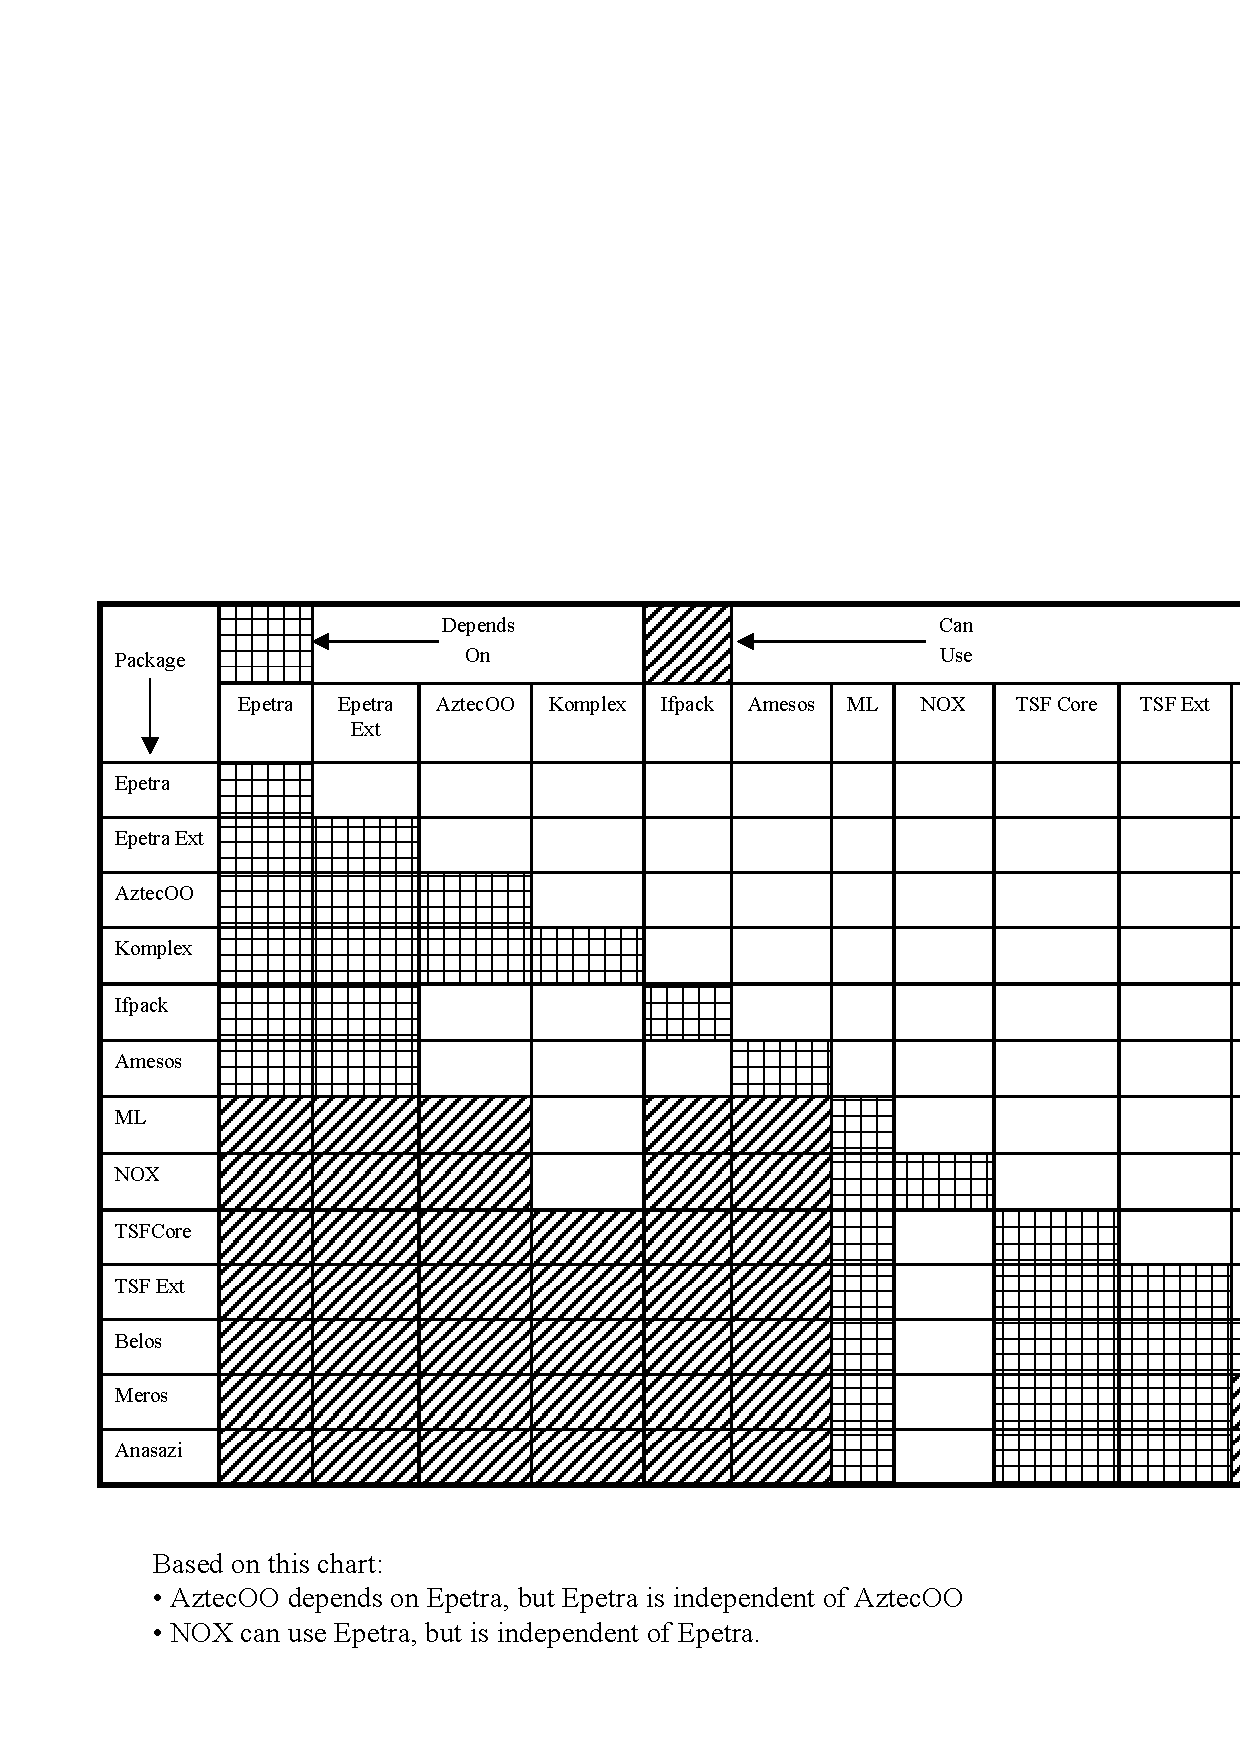
\includegraphics[height=8in]{../CommonFiles/TrilinosPackageDependencies}
%\end{center}
\label{Figure:TrilinosPackageDependencies}
\caption{Current Trilinos Package Dependencies}
\end{figure}
collection of Trilinos packages depend on each other.

%\section{Platform Portablility}
%	**(List platforms - encourage script submission)**

\clearpage
\bibliographystyle{plain}
\bibliography{TrilinosUserGuide}
\addcontentsline{toc}{section}{References}

\appendix
\section{Commonly Used CVS Commands}
\label{Section:CVS}
\begin{itemize}
\item {\bf Checking Out a Working Copy:}
To get started, checkout a working copy of the development branch from the CVS 
repository.  (Releases branches can be obtained by by checking out the 
appropriate tagged version of the repository.  More about this below.)

\DisplayCommand{cvs checkout Trilinos}

\item {\bf Updating a Working Copy:}
To update after a version has been obtained use the \InlineCommand{cvs update} 
command.  First, cd to the directory that is to be updated (often the 
Trilinos root directory).  Then type:

\DisplayCommand{cvs -q update -dP}

The ``-q'' option means ``be somewhat quiet''.  Try an update without the 
``-q'' to see exactly what the option does.  

The ``-d'' option means to get any new directories.  For example, if a new 
package is added to the repository, but the ``-d'' option is not used, that 
new package will never appear in the working copy.  However, the first time 
that the ``-d'' option is used, all of the new package directories will be 
downloaded, and from that time on, all CVS updates will update the 
directories that were downloaded.  It is good practice to include this 
option for every CVS update.

Finally the ``-P'' option ``prunes'' empty directories.  This helps to keep 
the directory structure from getting more cluttered than it needs to.  For 
example, the old ``petra'' and ``tsf'' packages were removed from the 
repository, but the directory structures will remain if this option is not 
specified.  If an empty directory is needed, simply issue one update 
command without the ``-P'' and the empty directories will be restored.

%\item{Working with Branches}
%cvs status

\end{itemize}

%\section{Common Bugzilla Tasks}
%\label{Section:BugzillaTasks}

\end{document}
